% Build from the repository root:
%   rsvg-convert -f pdf -o report/nus_logo.pdf report/nus_logo.svg
%   tectonic team32_final_report.tex
% The A4 cover follows T102_Group3_Final-Report(2).docx; the report body uses
% NeurIPS-like single-column, 10-point Times typography. References start on
% a separate page and do not count toward the 5--8-page report limit.
\documentclass[10pt,a4paper]{article}
\usepackage[a4paper,margin=1in]{geometry}
\usepackage{newtxtext,newtxmath}
\usepackage{microtype}
\usepackage{amsmath}
\usepackage{graphicx}
\usepackage{float}
\usepackage{booktabs}
\usepackage{array}
\usepackage{caption}
\usepackage[hidelinks]{hyperref}

\setlength{\parindent}{1em}
\setlength{\parskip}{0pt}
\setlength{\textfloatsep}{10pt plus 2pt minus 2pt}
\setlength{\intextsep}{9pt plus 2pt minus 2pt}
\captionsetup{font=small,labelfont=bf}
\renewcommand{\arraystretch}{1.08}
\hypersetup{pdftitle={Observation-Driven Grasping and Object-Aware Maze Traversal},
            pdfauthor={Nguyen Thien Duc, Team 32}}

\begin{document}
\begin{titlepage}
  \thispagestyle{empty}
  \centering
  \vspace*{-0.18in}
  {\bfseries\large Final Project\par}
  \vspace{0.18in}
  {\large Intelligent Robots: Algorithms and Systems\par}
  \vspace{0.30in}
  % The original SVG has transparent padding; trim only its PDF page margins.
  
\includegraphics[width=3.70in,trim=104bp 141bp 103bp 142bp,clip]{report/nus_logo.pdf}\par
  \vspace{0.30in}
  {\LARGE\bfseries Observation-Driven Grasping and\par
   Object-Aware Maze Traversal\par}
  \vspace{0.25in}
  {\large CS4278 / CS5478 Intelligent Robots\par}
  \vspace{0.12in}
  {\large Final Project Report\par}
  \vspace{0.12in}
  {\large AY 2026/2027 Semester 1\par}
  \vspace{0.12in}
  {\large Team 32\par}
  \vspace{0.30in}
  {\large\bfseries Submitted by\par}
  \vspace{0.12in}
  {\large Nguyen Thien Duc\quad A0287222E\par}
\end{titlepage}

% NeurIPS papers use compact, single-column 10-point Times text. The supplied
% reference cover is A4, so retain A4 here rather than switching paper size.
\newgeometry{top=0.83in,bottom=0.82in,left=1.24in,right=1.24in}
\pagestyle{plain}
\setcounter{page}{2}

\begin{center}
  {\Large\bfseries Observation-Driven Grasping and Object-Aware Maze Traversal}\par
  \vspace{4pt}
  Nguyen Thien Duc \quad Team 32 \quad CS4278 / CS5478
\end{center}
\vspace{-7pt}
\begin{abstract}
We present a complete controller for the provided Fetch pick--navigate--reach
task. From object points, surface normals, robot state, observed maze walls and
the goal, it selects a shape-aware grasp, executes collision-checked arm motion,
chooses a corridor-compatible carry pose and routes the combined robot--object
footprint. On 15 provided objects and ten development seeds per object, the
automatic controller lifted and held 145/150 objects and delivered 135/150
within the 10\,cm goal tolerance. Successful pickups comprise 117 ordinary
top-down, nine bowl-rim and 19 side/edge grasps; ten of the 15 end-to-end
failures were transport drops. These are seeded evaluations of the supplied
environment, not estimates of performance on hidden objects or mazes.
\end{abstract}

\section{Problem and design choices}
The course task asks a Fetch mobile manipulator to pick a provided YCB-derived
object from a table, carry it through a wall maze and bring its center within
0.10\,m of a three-dimensional goal~\cite{course,ycb}. The simulator accepts
absolute position targets for 15 controllable joints. Its observations include
1,024 object surface samples and outward normals, current joint state, object
and goal poses, and the XY positions of wall cubes. The policy does not read a
precomputed solution path or attach an object to the gripper.

Pickup success alone is not sufficient: a grip that lifts a bowl may peel off
its rim, and a grip that holds a hammer at the table may lose it when the arm
stows. We consequently evaluate the grasp after a 10\,cm lift and a 50-step
hold, then monitor the same physical hold throughout navigation. A valid
delivery additionally requires a goal-distance check after a final 50-step
hold. Figure~\ref{fig:scene} illustrates the geometry addressed by the
controller.

\begin{figure}[H]
  \centering
  \includegraphics[width=.82\linewidth]{imgs/scene.png}
  \caption{Provided scene: the robot must move a grasped object from the table
  through observed walls to the goal. The route is checked for both the robot
  and the held object's footprint.}
  \label{fig:scene}
\end{figure}

Our solution has three coupled decisions: find contacts that fit the jaws and
are reachable without hitting the table; move the hand to a carry pose that
fits the maze; and route the base while accounting for the object's measured
offset. This coupling matters especially for wide, rimmed and flat objects.

\section{Observation-driven grasp selection}
\subsection{Contact proposals and executable arm motion}
We deterministically subsample at most 256 of the 1,024 observed surface
points, then propose nearly horizontal, opposing contact pairs. For two points
$p_i,p_j$ with outward normals $n_i,n_j$, let
\begin{equation}
 u=\frac{p_j-p_i}{\lVert p_j-p_i\rVert},\qquad
 (-n_i)\!\cdot u>0.85,\quad n_j\!\cdot u>0.85 .
 \label{eq:contacts}
\end{equation}
Pair height difference is below 18\,mm and width is normally below 85\,mm;
the threshold can rise to 100\,mm for observed wide objects. Candidate
scores favor opposing alignment and penalize displacement from the observed
center. After near-duplicate suppression, the planner tries at most 30
different grasps. This antipodal-style construction is motivated by classical
grasp geometry and point-cloud grasp detection~\cite{nguyen,tenpas}; the
alignment test is a heuristic, \emph{not} a proof of force closure.

For each candidate, the controller solves wrist pose and arm joint targets in
an isolated PyBullet kinematics client. It checks the planned joint segments
at intermediate configurations against the table and rejects an approach
whose gripper palm contacts the object before its fingers can close. The live
robot only receives joint-position commands; table clearance, joint motion
and finger proximity are checked again during execution. We approach from
above by default and use a near-flank side pinch for geometries such as the
wide Master Chef can. A long, flat object with a narrow handle is tried from
above first: the hammer's broad head would otherwise trigger a side approach
that lifts but can rotate free during transport.

\subsection{Rim and plate are distinct geometries}
Ordinary opposing sidewalls do not describe a thin bowl rim. For a bowl-like
point cloud, we seek nearby inner/outer rim samples with opposing local
normals and support on both walls. The gripper approaches this radial pair
from above, matches its closure to rim thickness and lifts in short,
straight-up Cartesian IK segments. A long joint-space interpolation could
sweep the wrist laterally and peel the rim out of the jaws.

A plate lying flush with the table has no clearance for a lower finger.
After direct plans fail, a geometry-triggered fallback pushes it toward the
observed table edge with closed fingers, obtains a fresh point cloud and
pinches the newly exposed lip with one finger above and one below. The plate
is never teleported or rigidly attached. Figure~\ref{fig:plate} depicts the
result of the staged pickup.
\begin{figure}[H]
  \centering
  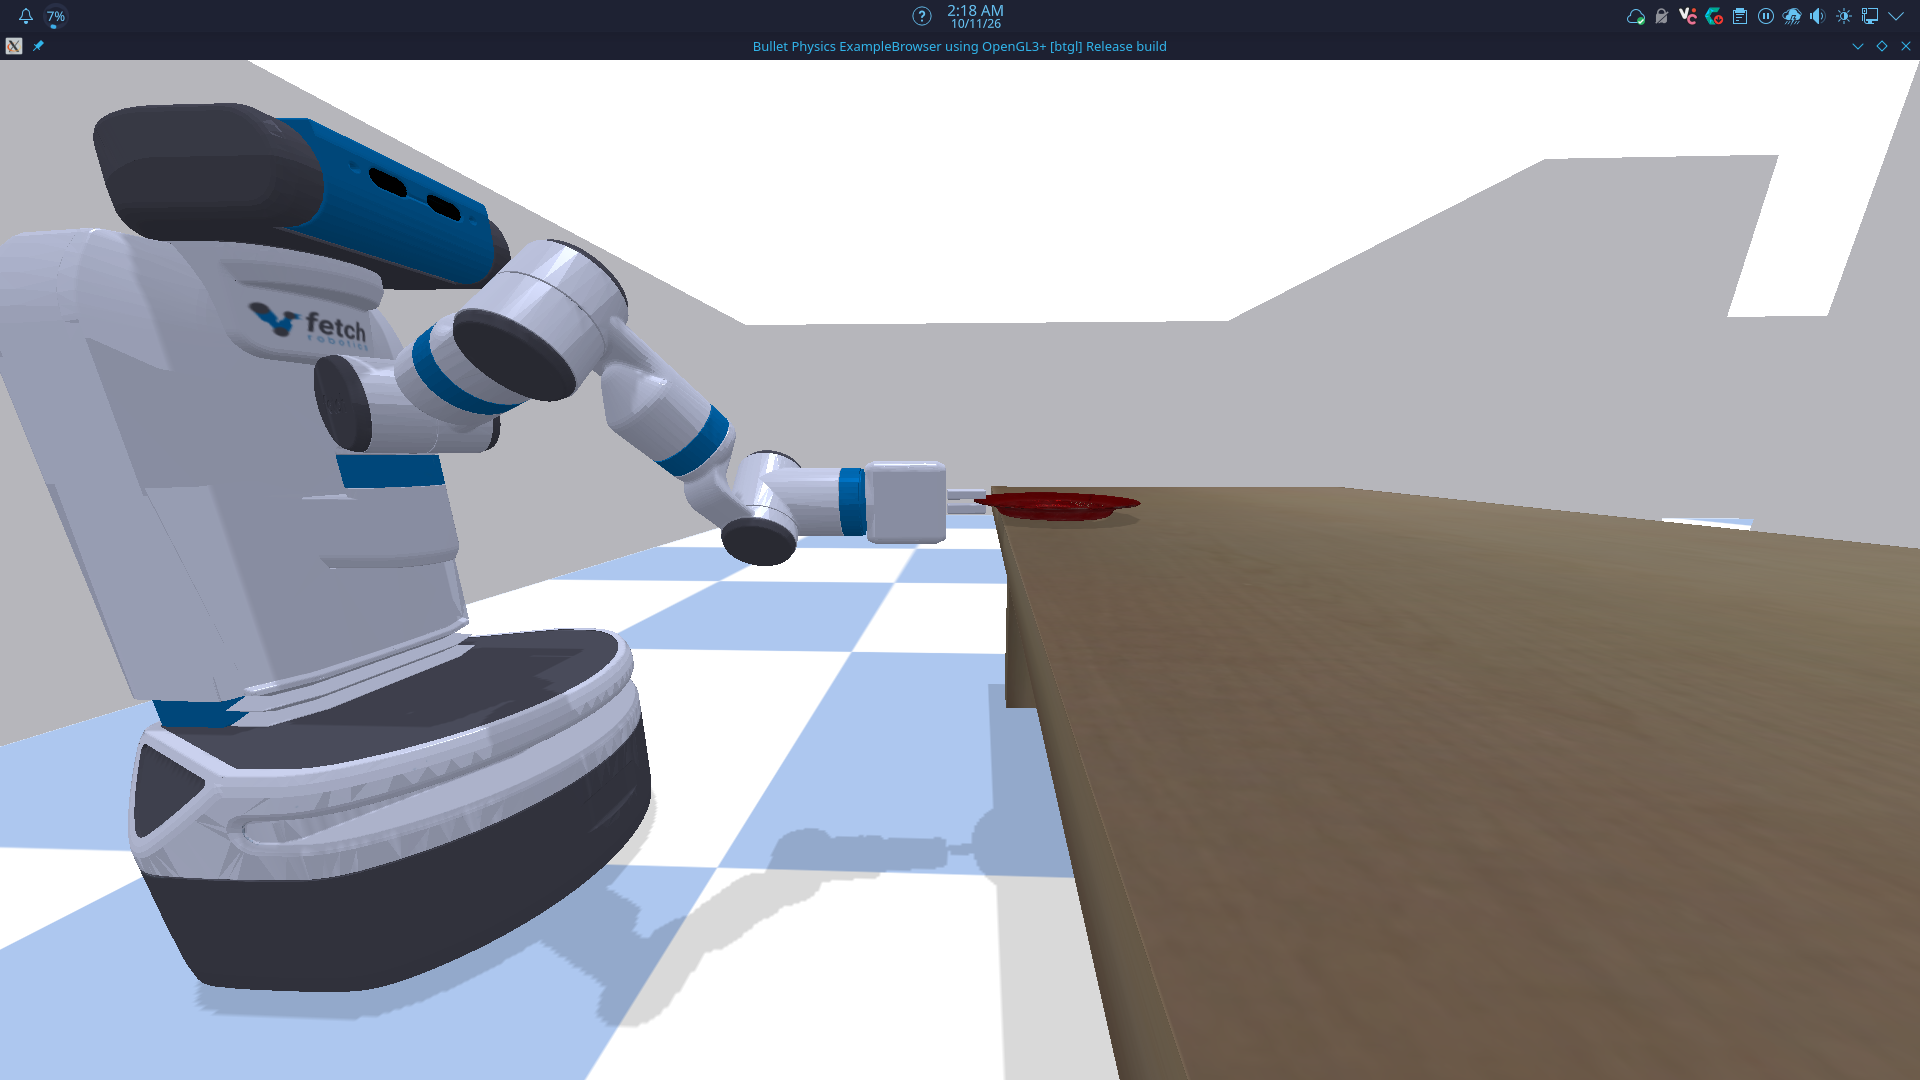
\includegraphics[width=.66\linewidth]{imgs/plate_grasp.png}
  \caption{The physically staged plate exposes an edge for an upper/lower
  side pinch. Its initial flush pose cannot be gripped this way.}
  \label{fig:plate}
\end{figure}

\section{Carrying, mapping and reaching}
After a measured lift, the controller may roll a top-down grasp in safe
15-degree increments to give one jaw better support; long thin objects are
limited to one such increment. It searches IK-valid stow poses with the held
object close to the base. Each candidate is accepted only if its projected
robot--object footprint admits a collision-checked maze route. Thus the carry
pose is chosen \emph{before} committing to the wall-grid plan; a successful
table pickup cannot by itself guarantee a traversable carried configuration.

We construct a two-dimensional grid from the observed wall positions. Let
$b$ denote base XY, $\delta$ the measured object-center offset from the base,
$B$ the robot's observed XY collision bounds and $O$ the carried object's
observed XY half-extents. A base location is admissible only if the translated
base bounds $b+B$ and object bounds $b+\delta+O$ both clear the walls (with a
small margin). A* searches neighboring free cells and only shortcuts between
waypoints when the full segment is free~\cite{hart}. The nominal goal-base
position is $b^*=g_{xy}-\delta$; it may be shifted slightly within the goal
tolerance when the corridor exit requires clearance. During motion we check
live robot and object wall distances as well as the object--hand displacement.

At the exit, the arm adjusts the held object's height and the base trims small
XY errors before the final goal and hold check. A staged plate can leave the
arm folded near several joint limits: if no ordinary collision-free final
lowering pose exists, a plate-only fallback first verifies a 0.5\,m retreat
through open space, then extends and lowers the grasp while preserving jaw
closure. This resolves a reachability problem without requiring a wall
collision or an object release.
\begin{figure}[H]
  \centering
  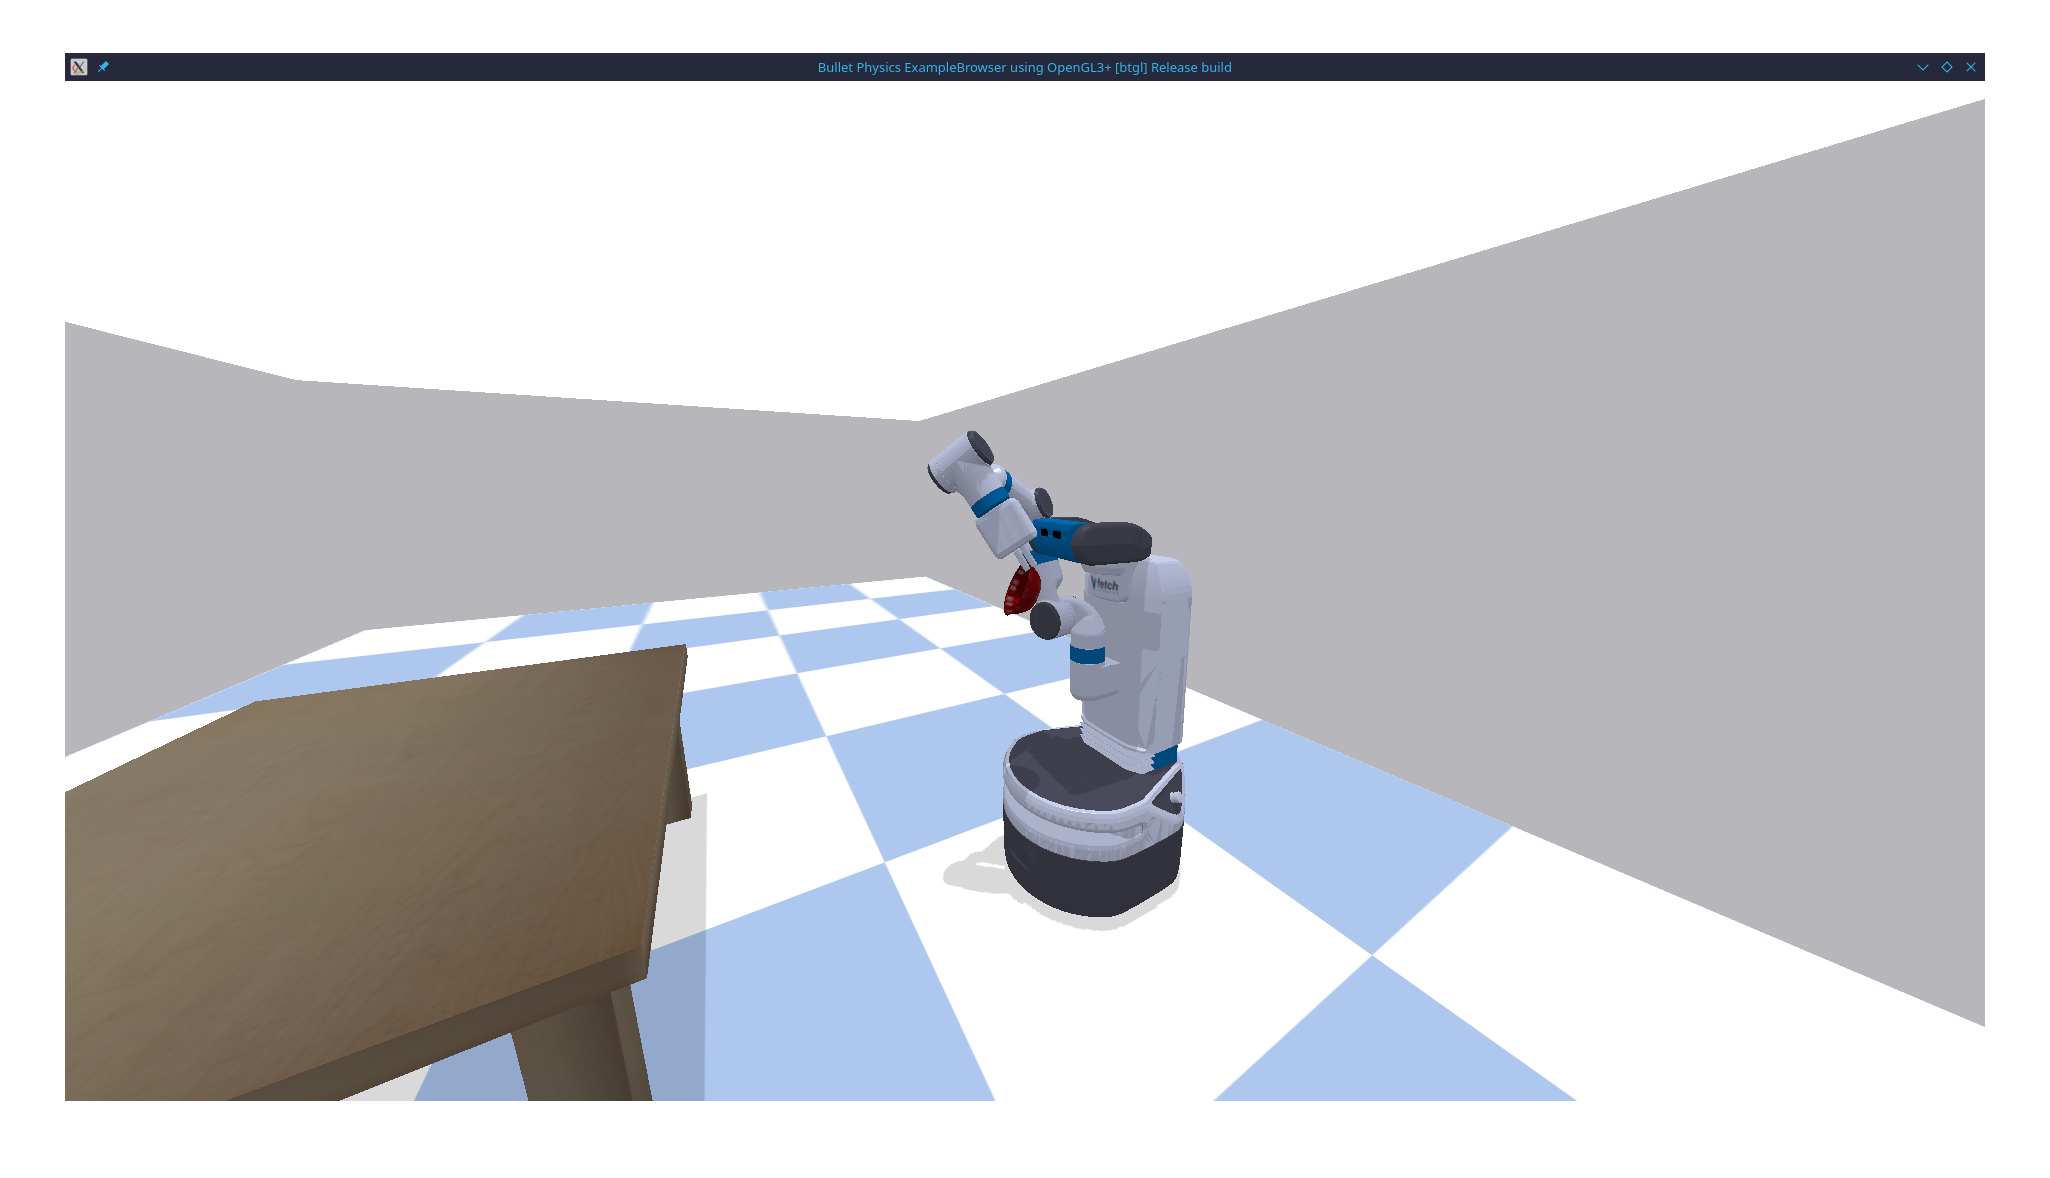
\includegraphics[width=.66\linewidth]{imgs/carry_pose.png}
  \caption{A measured carry pose stows the held object close to the base before
  the robot enters the wall grid; the grid subsequently protects both.}
  \label{fig:carry}
\end{figure}

\section{Evaluation and results}
\subsection{Protocol and aggregate outcomes}
We ran independent headless trials for all 15 supplied object types and seeds
60--69: 150 attempts in each pickup-only and full-task benchmark, with 24
worker processes. Each run starts from a fresh simulator, settles the object
for 80 environment steps, then executes the automatic policy. The maze wall
generator uses a fixed internal seed; trial seeds change the sampled object
surface and randomized entry/exit rows. Hence this is a \emph{development-seed}
evaluation, not a hidden-maze test. A pickup must rise at least 0.10\,m and
survive 50 held steps; end-to-end success must also pass the simulator's
3D goal test after transport. An environment step can contain several Bullet
physics ticks; reported timings below count environment steps.

\begin{table}[H]
\centering\small
\caption{Successful pickups and full deliveries per object (10 seeds each).
Bowl-rim grasps are counted under the benchmark's top-down label.}
\label{tab:objects}
\begin{tabular}{@{}lrr@{\hspace{.38in}}lrr@{}}
\toprule
Object & Pick & Goal & Object & Pick & Goal\\
\midrule
Chef can & 9 & 8 & Bleach & 9 & 8\\
Sugar box & 10 & 8 & Bowl & 9 & 9\\
Soup can & 10 & 10 & Mug & 10 & 10\\
Mustard & 10 & 10 & Plate & 10 & 8\\
Potted meat & 10 & 10 & Large marker & 10 & 10\\
Banana & 10 & 8 & Hammer & 8 & 7\\
Strawberry & 10 & 10 & Foam brick & 10 & 10\\
Apple & 10 & 9 & & & \\
\midrule
\multicolumn{4}{@{}l}{\textbf{Total across 150 trials}} & \textbf{145} & \textbf{135}\\
\bottomrule
\end{tabular}
\end{table}

The controller picked up \textbf{145/150} and delivered \textbf{135/150}.
Successful pickups were 117 ordinary top-down, nine bowl-rim top-down and
19 side grasps (nine can, ten staged plate). This partitions the 145 holds;
the benchmark's coarser labels are 126 top-down and 19 side. Five pickups
failed: three objects did not lift and two approaches stopped at a table
clearance guard. Among successful pickups, ten objects subsequently dropped
during transport; no final-reach-pose failures remained in this cohort.
Table~\ref{tab:objects} gives the per-object results. Median first-lift time
among successful pickup trials was 1,613 environment steps. Median navigation
time among delivered trials was 4,041 steps, and every successful navigation
finished below the 15,000-step limit.

\subsection{What changed and what did not}
On the same seeds, an early pickup version held 126/150; adding local bowl-rim
grasps raised this to 135/150, and staged plate pickup reached 142/150 in an
intermediate version. The latest policy holds 145/150. These development
iterations are not independent comparisons or hidden-test estimates. For a
separate \emph{historical paired} carry-pose ablation, a full 180-degree
palm-up flip delivered 87/150 versus 128/150 for the then-default small
jaw-roll policy. Both used 142 successful pickups, and the palm-up version
frequently lacked a safe turning pose; those figures precede the present
plate and hammer changes and must not be compared as current policies.

The latest hammer policy prioritizes the narrow handle rather than a side
pinch caused by its broad head. It turns seeds 63 and 68 from transport drops
into deliveries; hammer delivery is now 7/10 rather than 5/10, while other
object outcomes in this cohort are unchanged. The plate's 10/10 pickups give
8/10 deliveries, including three rescued by the guarded final-reach retreat;
its remaining two trials drop during transport.

\subsection{Diagnosing the remaining failures}
The ten transport drops comprise two each for the sugar box, banana and
plate, and one each for the Master Chef can, bleach cleanser, apple and
hammer. The live monitor marks a lost grasp when the object deviates more
than 0.12\,m from its hand-relative position or falls more than 0.12\,m below
its carried height. These are observations of failed retention, not evidence
that A* selected an unsafe maze route. The five earlier pickup failures
divide into three objects not lifted (two hammers and one bowl) and two
table-clearance stops (one can and one bleach cleanser). No successful
pickup failed because a wall route or final reach pose was unavailable in
this particular cohort.

End-to-end success \emph{given pickup} is $135/145=93.1\%$. This conditional
rate explains why improvements at the pickup stage need not translate
directly into delivered objects: a plate can survive the table lift yet
shift inside the jaws during stowing. Conversely, a tiny grasp-planning
change can matter greatly downstream: the two hammer seeds that switched
from a wide side pinch to a narrow top-down handle pinch retained the object
throughout the maze, even though the number of successful hammer lifts
remained 8/10.

\subsection{Interpretation of the policy iterations}
Table~\ref{tab:iterations} records the pickup-stage development sequence.
The counts use the same provided objects and seeds, but the controllers were
changed between rows; the increments are engineering history rather than
confidence intervals or independently randomized trials. The first large
gain came from treating a thin rim as a pair of \emph{local} opposing walls,
not as the whole bowl width. The next gain required moving the plate to create
an accessible contact, rather than changing an IK tolerance until an unsafe
table-level pinch looked feasible. The latest successful pickup count stayed
at 145 when hammer selection changed: selecting a better hold improved
\emph{delivery}, not the number of objects initially lifted.

\begin{table}[H]
\centering\small
\caption{Pickup-policy development on the same 150 provided-object trials.
The last row is the report's current 24-worker benchmark.}
\label{tab:iterations}
\begin{tabular}{@{}lr@{}}
\toprule
Automatic pickup policy & Held after lift + 50 steps\\
\midrule
Initial antipodal and IK policy & 126/150\\
Add inner/outer bowl-rim lift & 135/150\\
Add staged plate-edge pickup (intermediate) & 142/150\\
Latest geometry-specific pickup and grasp selection & 145/150\\
\bottomrule
\end{tabular}
\end{table}

The aggregate lift-time median also conceals a practical tradeoff. Most
successful lifts clear the 10\,cm threshold relatively quickly, but every
plate trial in this cohort uses many short, checked motions for the physical
slide, reobservation and edge pinch. Their median is 5,576 environment steps,
well beyond the course's 3,000-step pickup target. The gripper is kept close
to the table during this procedure, so simply issuing a larger or faster
joint command would remove the safeguards that prevent fingertip and wrist
collisions. Reducing redundant staging movement while retaining measured
clearance is a more defensible performance target than weakening collision
checks. These timing observations are from simulator actions, not wall-clock
seconds or a hardware Fetch robot.

Finally, the ablation on full palm-up turning does not isolate a universal
``best orientation'': it tested a different pickup policy and older plate
behavior. Its useful causal observation is narrower. A large wrist flip
often has no safe arm pose and can destabilize otherwise held objects; a
small, checked roll is easier to preserve while moving into the maze. We
therefore report that earlier comparison separately instead of combining
its 87/150 and 128/150 deliveries with today's 135/150 result.

\section{Limitations and conclusion}
The remaining 15 unsuccessful full trials include five pickup failures and
ten transport drops, so reliable lifting does not imply reliable placement.
Two hammer seeds still do not lift, and one hammer seed still drops in transit.
The plate's median successful lift takes 5,576 environment steps, above the
course's 3,000-step pickup timing target even though all ten plate pickups
succeed. The controller relies on sampled surface geometry, fixed-heading
base translation, approximate footprint bounds and a fixed-maze generator;
we have not established robustness to unseen object poses, obstacle layouts
or sensor noise. Its contact checks are heuristics rather than a force-closure
or global motion-planning guarantee.

The bounded grasp search still spends time on many alternative contact
pairs and IK branches. Each geometric proposal is evaluated against a
kinematic model, while the executed robot can lag commanded joint targets.
This is why we check measured pose and clearance during motion rather than
trusting collision-free IK endpoints alone. The finite sampled surface may
also miss an exposed contact, and axis-aligned object bounds can overstate
clearance needs for rotated shapes. Both choices favor safety on these
provided scenes but can cause avoidable failures on different layouts.

The main result is an end-to-end lesson: selecting contacts, moving safely to
a grasp, choosing a carry pose and routing the held object are inseparable.
Rim-aware lifting and staged edge exposure address geometry at the table;
object-aware A* and a guarded open-space final reach preserve delivery.
Across the provided evaluation cohort this yields 145/150 measured pickups
and 135/150 full deliveries, with remaining work concentrated in grip
retention and the slow plate staging sequence.

\subsection*{Reproducibility}
The trial-level reports in \texttt{presentation/} are:
\begin{itemize}
\setlength{\itemsep}{0pt}
\item \texttt{pickup\_benchmark\_latest.json} (pickup);
\item \texttt{full\_task\_benchmark\_latest.json} (delivery).
\end{itemize}
From the repository root, run
\texttt{benchmark\_pickup.py} or \texttt{benchmark\_full\_task.py}
with \texttt{--seeds 60 61 62 63 64 65 66 67 68 69 --workers 24}.
Both report per-object outcomes and individual failure reasons. The supplied
environment and our controller sources accompany this report; no claim is
made about the five unprovided course evaluation seeds.

\clearpage
\begin{thebibliography}{9}\small\raggedright
\bibitem{course} NUS-LinS-Lab. \emph{Pick-Navigation-Reach Default Project},
CS4278/CS5478 course environment and rubric, project repository and supplied
task brief. \url{https://github.com/NUS-LinS-Lab/Pick-Nav-Reach-Default-Project}.

\bibitem{nguyen} V.-D. Nguyen. Constructing force-closure grasps.
\emph{The International Journal of Robotics Research}, 7(3):3--16, 1988.

\bibitem{tenpas} A. ten Pas and R. Platt. Using geometry to detect grasp
poses in 3D point clouds. In \emph{International Symposium on Robotics
Research}, 2015.

\bibitem{hart} P. E. Hart, N. J. Nilsson, and B. Raphael. A formal basis
for the heuristic determination of minimum cost paths. \emph{IEEE
Transactions on Systems Science and Cybernetics}, 4(2):100--107, 1968.

\bibitem{ycb} B. Calli, A. Walsman, A. Singh, S. Srinivasa, P. Abbeel,
and A. M. Dollar. Benchmarking in manipulation research: The YCB object
and model set. \emph{IEEE Robotics \& Automation Magazine}, 22(3):36--52,
2015. \url{https://www.ycbbenchmarks.com/}.

\bibitem{bullet} E. Coumans and Y. Bai. \emph{PyBullet: A Python Module for
Physics Simulation for Games, Robotics and Machine Learning}.
\url{https://pybullet.org/}, 2016--2021.
\end{thebibliography}
\end{document}
